% My answer for http://tex.stackexchange.com/q/266206/828
% Direct link: http://tex.stackexchange.com/a/266218/828
\documentclass{standalone}

\usepackage{tikz}

\begin{document}

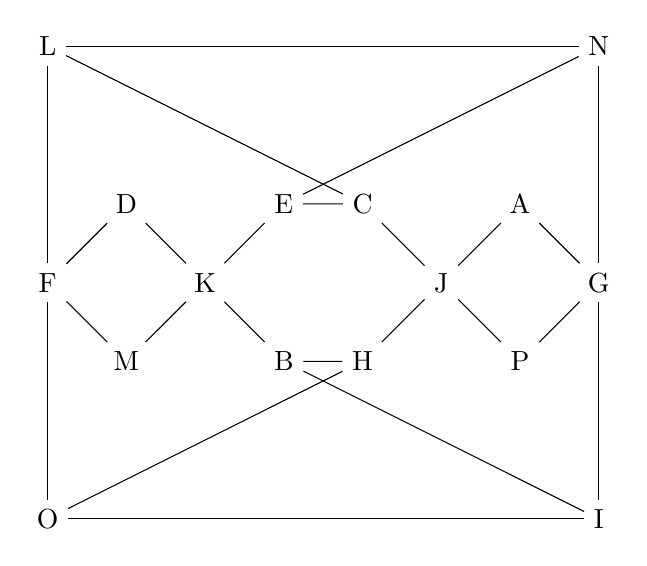
\begin{tikzpicture}
	% left
	\node (f) at (0,0) {F};
	\node (d) at (1,1) {D};
	\node (k) at (2,0) {K};
	\node (m) at (1,-1) {M};
	% middle
	\node (e) at (3,1) {E};
	\node (c) at (4,1) {C};
	\node (b) at (3,-1) {B};
	\node (h) at (4,-1) {H};
	% right
	\node (j) at (5,0) {J};
	\node (a) at (6,1) {A};
	\node (g) at (7,0) {G};
	\node (p) at (6,-1) {P};
	% outer
	\node (l) at (0,3) {L};
	\node (n) at (7,3) {N};
	\node (o) at (0,-3) {O};
	\node (i) at (7,-3) {I};
	% connections
	\draw (f) -- (d) -- (k) --(m) -- (f);
	\draw (k) -- (e) -- (c) -- (j);
	\draw (k) -- (b) -- (h) -- (j);
	\draw (j) -- (a) -- (g) --(p) -- (j);
	\draw (f) -- (l) -- (n) -- (g) -- (i) -- (o) -- (f);
	\draw (l) -- (c);
	\draw (e) -- (n);
	\draw (o) -- (h);
	\draw (b) -- (i);
\end{tikzpicture}

\end{document}